
\section{Gas targets}\label{gastarg}

\subsection{Windowless targets and differential pumping}


For our purpose of measuring proton or alpha radiative capture in inverse kinematics, a hydrogen or helium gas target is required which has sufficient density  to contain energetically the targeted resonance width or a sufficient direct capture interval to provide a measurable yield. Additionally, the uncertainty of a resonance position --- from transfer reaction measurements and nuclear mass information --- has to be taken into account. As the resonant yield is inverse proportional to the target stopping power it is also beneficial to avoid inactive nuclei in its composition, {\it e.g.} a pure hydrogen target provides a factor 3--4 higher yield than a CH$_2$ foil target.  A gas target is also virtually indestructible and stable in its composition while in plastic foil targets the carbon to hydrogen ratio is known to change even under modest heavy ion beam flux of the order of $10^7 \unit{s^{-1}}$.\\
In order to achieve a target thickness of 10 keV (in the centre-of-mass system) with the light to medium mass ion beams in question at astrophysically relevant energies, a target number density of approximately $5\cdot10^{18} \unit{nuclei/cm^2}$ of hydrogen is required. To provide unimpeded beam and recoil transmission, the gas cannot be confined by foil windows, leaving as the only possible approach the use of a windowless, differentially pumped gas target. The gas pressure necessary to achieve the required target number density is given by the formula \cite{rolf88} 
\begin{equation}
n_A = 9.66\cdot10^{18} x \nu \frac{p}{T} \mathrm{[1/cm^2]}
\end{equation}
with $x$ the target length in cm, $\nu$ the number of atoms per molecule, $p$ the pressure in Torr, and $T$ the temperature in K.\\
It should be noted that the target length needs to be kept small ($<$ 10--15 cm) in order not to significantly increase the acceptance requirements for the recoil separator. The windowless approach means that a target pressure of a few torr needs to be maintained in the gas cell, but a reduction to the order of $10^{-6} \unit{Torr}$ achieved over several gas flow limiting apertures and pumping stages is necessary to allow connection to the accelerator and separator. On the accelerator side the dimensions of these apertures are defined typically by the beam dimensions, while on the separator side the reaction recoil cone needs to be accommodated. Therefore, it is preferable to compress the length of the differential pumping stages as much as possible to allow for smaller aperture sizes. A typical pumping scheme is depicted in Fig. \ref{fig:dragon_pumping}.
\begin{figure}
\resizebox{0.9\columnwidth}{!}{
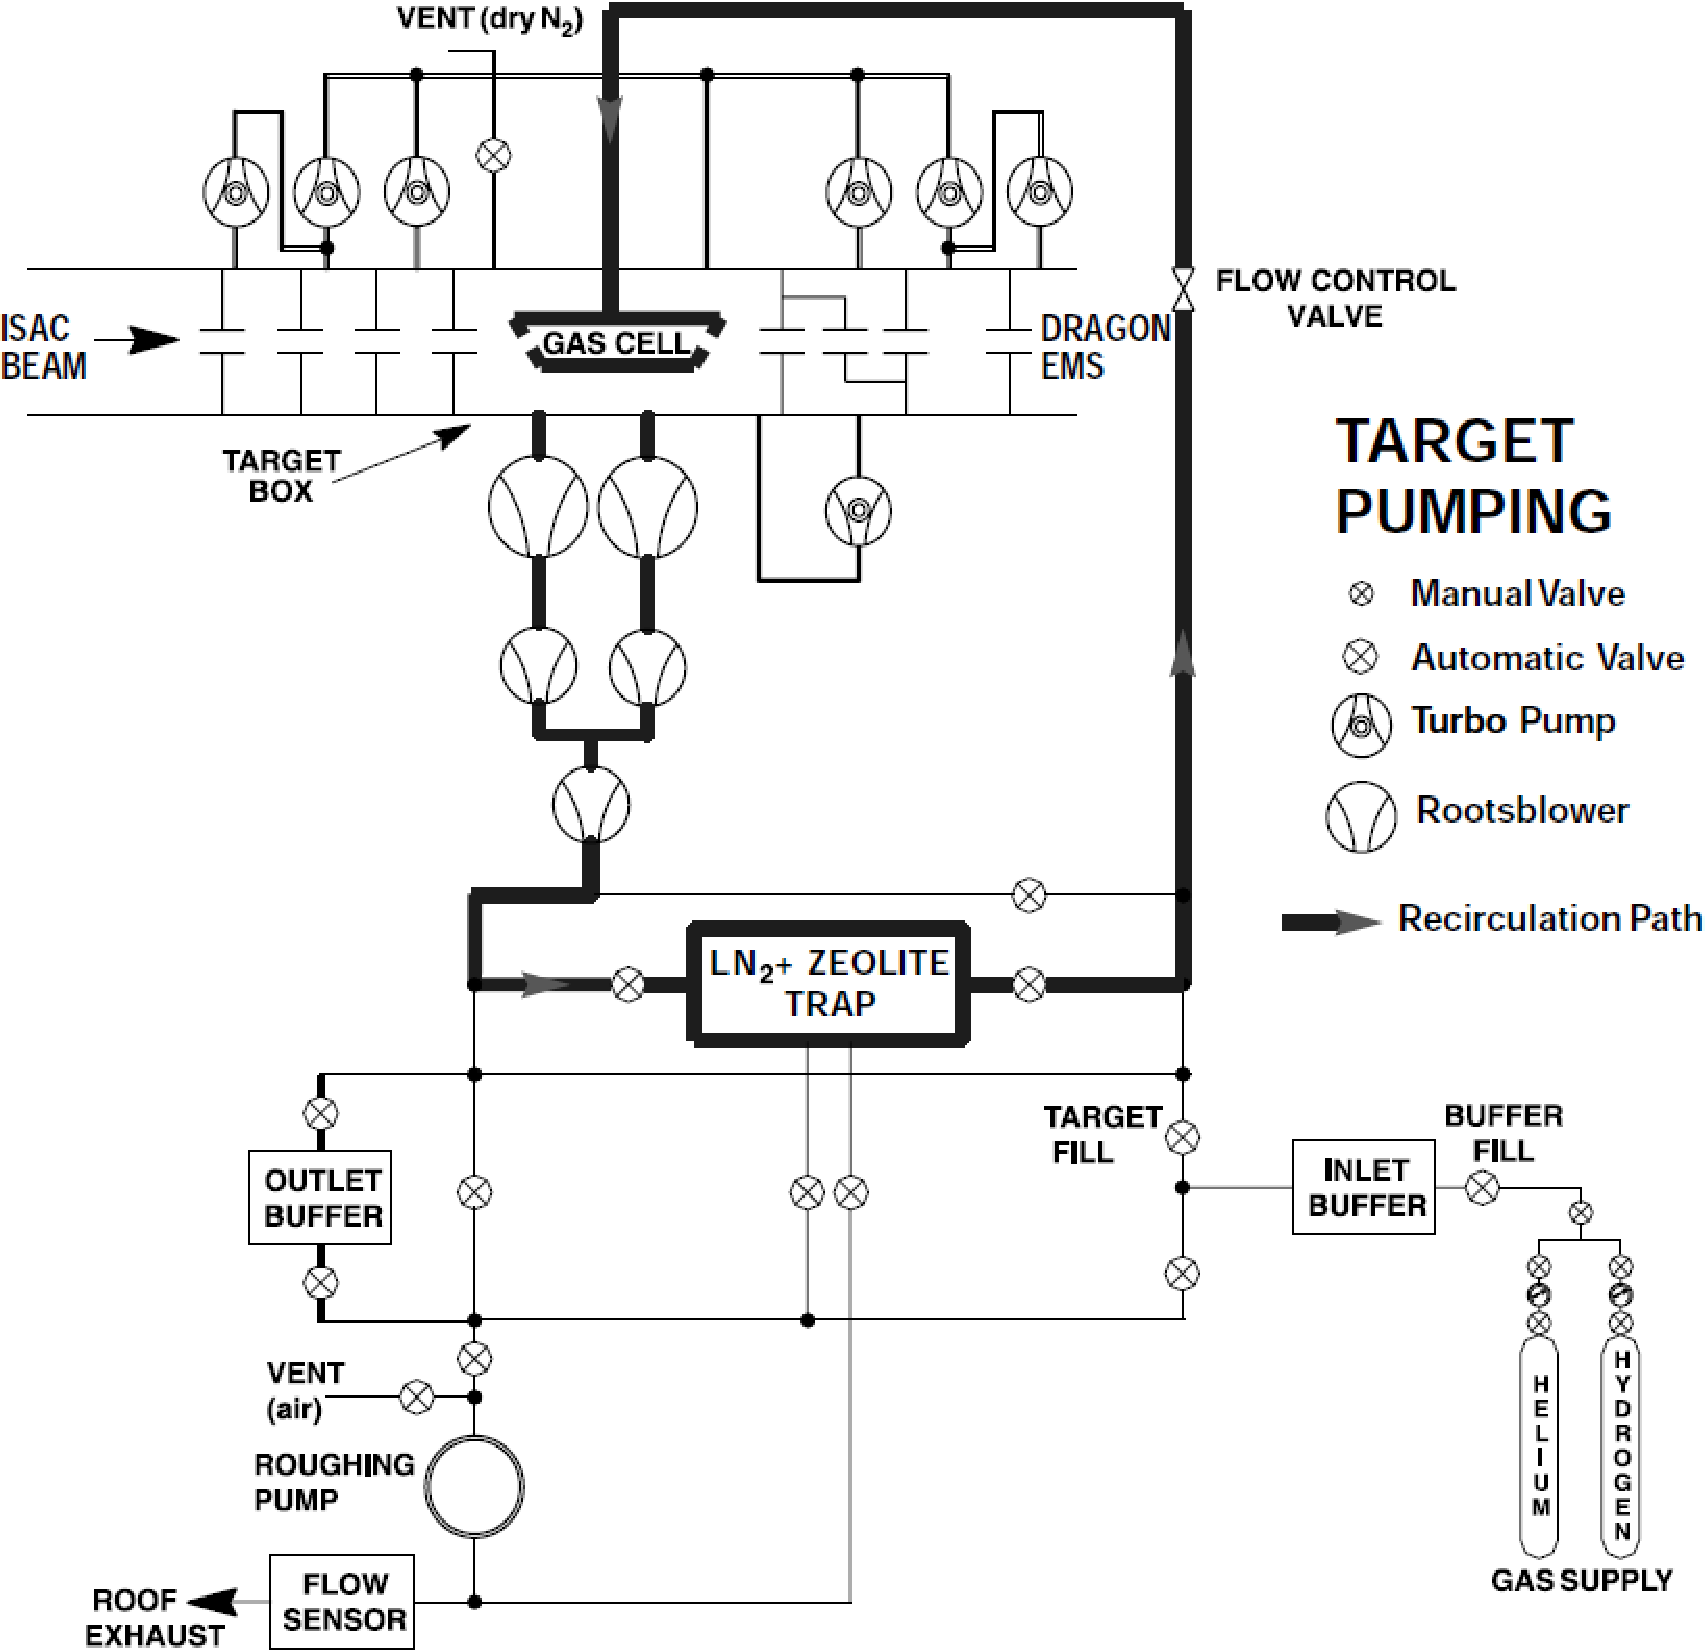
\includegraphics{Hutcheon03_Fig5_DRAGON-gastargetpumps}
}
%\vspace{5cm}       % Give the correct figure height in cm
\caption{DRAGON gas target pumping scheme. Taken from \cite{hutc03b}.}
\label{fig:dragon_pumping}
\end{figure}
\emph{[Figure of pumping scheme]} \\
For the extraction of a cross section or resonance strength from the measured yield we require knowledge of the stopping power of the heavy ions in hydrogen or helium. While these are typically taken from the widely used SRIM code \cite{zieg}, recent experiments \cite{grei04} have shown deviations of the order of 20--30 \% from the semi-empirical values. Therefore, direct measurement of the respective stopping power should, where possible, be preferred. Additionally, angle and energy scattering of the beam and recoils on their way through the target gas need to be estimated and taken into account in the calculation of the required recoil separator acceptance. While the ions pass the gas they also undergo charge-changing collisions. If the target is thick enough, an equilibrium charge state distribution is achieved (semi-empirical description available in {\it e.g.} \cite{liu03}). However, if the reaction recoil originates from the downstream side of the gas target, the remaining gas track length is not sufficient to reach this equilibrium, and it is advisable to obtain the charge state distribution by tuning the recoil separator for measurements of the several charge states expected to be most abundant.\\
Especially for the astrophysically most important reactions \nuc{12}{C}\reac{\alpha}{\gamma}\nuc{16}{O} and \nuc{15}{O}\reac{\alpha}{\gamma}\nuc{19}{Ne}, the recoil cone angles are quite demanding on separator acceptance. In order not to alleviate \emph{[alleviate? do you mean aggravate?]} the problem through the use of an extended gas target length of 5 -- 10 cm, recent discussions propose the use of a gas jet target with approximately 4 -- 5 mm jet diameter matched to the dimension of the incoming ion beam. As can be seen in the pumping scheme \emph{[gas jet target pumping scheme figure]} for an appropriate gas jet target ($\approx 5\cdot10^{18} \unit{cm^{-1}}$ areal density), such a setup (which is in its early construction phases for deployment at Oak Ridge National Laboratory) requires significantly more powerful pumping stages as well as expensive gas compression and cleaning.\\
 

\small
\begin{itemize} 
\item What are the advantages of using a differentially pumped windowless gas target?
\item for our purpose H and He targets best solution as he not available implanted in sufficient densities; H possibles but about factor 4 yield advantage due to 1/stopping term in resonant yeild equation
\item also indestructible and stable in composition (plastic foils change and have current limit)
\item windows are detrimental to recoil transmission, therefor windowless, differentially pumped approach ideal for our application
\item what thickness to chooses: resonance width (usually small) + uncertainty in resonance position (info from transfer reactions plus knowledge of masses of reaction partners of order a few keV) follows target thickness of about 10 kev in CM system is useful leading areal target densities aspired of 5E18 1/cm2
\item at 7-8 Torr achieved with about 10 cm length
\item give equation from Rolfs for gas target density
\item  length of target determines origin of recoil; needs to be matched with acceptance of the recoil separator (shorter is better); some reactions would benefit from gas jet which is however technically more challenging due to the large gas flow rates involved.
\item Gas flow limiting apertures need to be matched to the heavy (radioactive) ion beam properties and the nuclear reaction recoil cone angle
\item we need to know stopping powers; found differences to SRIM of the order of 20-30% when we measured ourselves
\item energy and angle scattering needs to be estimated and included in acceptances; not well known
\item charge state distributions, often equilibrium not achieved; preferably to be measured in experiment
\end{itemize}
\normalsize


\subsection{Extended length and jet gas targets}
